

\section*{Introduction}

Quantitative mass spectrometry based spatial proteomics involves
elaborate, expensive and time consuming experimental protocols and
considerable effort is invested in the generation of such data.
Multiple research groups have described a variety of approaches to
establish high quality proteome-wide datasets (see for example
\cite{Gatto:2010} for a review, and
\cite{hyper,Itzhak:2016,Jean_Beltran:2016} for recent
examples). However, data analysis is as critical as data production
for reliable and insightful biological interpretation. Here, we walk
the reader through a typical pipeline for the analysis of such data
using several Bioconductor~\cite{Huber:2015} packages for the R
statistical programming environment.

The main package to analyse protein localisation data is
\Biocpkg{pRoloc}, which offers a set of dedicated functions for the
analysis of such data. \Biocpkg{pRoloc} itself relies on
\Biocpkg{MSnbase} to manipulate and process quantitative proteomics
data. Many other packages are used by \Biocpkg{pRoloc} for clustering,
classification and visualisation. Support for interactive
visualisation is offered by the \Biocpkg{pRolocGUI} package.

In this workflow, we will describe how to prepare the spatial
proteomics data starting from a spreadsheet containing quantitative
mass spectrometry data, through to some essential data processing
steps, and finish with different applications of machine learning
(Figure \ref{fig:overview}). We focus on a recent pluripotent mouse
embryonic stem cells experiment \cite{hyper}. These data, as well as
additional annotated and pre-formatted datasets from various species
are readily available in the \Biocexptpkg{pRolocdata} package.

Installation of Bioconductor package is documented in detail on the
\href{http://bioconductor.org/install/#install-bioconductor-packages}{Bioconductor
  installation help page}. Below, we show how to install the four main
packages used in this workflow:

\begin{Schunk}
\begin{Sinput}
> source("https://bioconductor.org/biocLite.R")
> biocLite(c("MSnase", "pRoloc", "pRolocdata", "pRolocGUI"))
\end{Sinput}
\end{Schunk}


This procedure is also applicable to any packages, from
\href{https://cran.r-project.org/}{CRAN} as well as GitHub. Once a
package has been installed, it needs to be loaded for its
functionality to become available in the R session; this is done with
the \texttt{library} function e.g.  to load the \Biocpkg{pRoloc} one
would type \texttt{library("pRoloc")} after installation.

If you have questions about this workflow in particular, or about
other Bioconductor packages in general, they are best asked on the
\href{https://support.bioconductor.org/}{Bioconductor support site}
following the
\href{http://www.bioconductor.org/help/support/posting-guide/}{posting
  guidelines}. Questions can be tagged with specific package names or
keywords. For more general information about mass spectrometry and
proteomics, the readers are invited to read the
\Biocexptpkg{RforProteomics} package vignettes and associated
papers \cite{Gatto:2014,Gatto:2015}.

\begin{figure}[!ht]
  \centering
  \includegraphics[width=.5\textwidth]{./Figures/overview.pdf}
  \caption{Schematic overview of the pRoloc pipeline from data import, through to data processing, machine learning and data export.}
  \label{fig:overview}
\end{figure}


\section*{Reading and processing spatial proteomics data}

\subsection*{The use-case: predicting sub-cellular localisation in pluripotent embryonic mouse stem cells}

As a use-case, we analyse a recent high-throughput spatial proteomics
dataset from pluripotent mouse embryonic stem cells (E14TG2a)
\cite{hyper}. The data was generated using hyperplexed LOPIT
(hyperLOPIT), a state-of-the-art method relying on improved
sub-cellular fractionation and more accurate quantitation, leading to
more reliable classification of protein localisation across the whole
sub-cellular space. The method uses an elaborate sub-cellular
fractionation scheme, enabled by the use of Tandem Mass Tag (TMT)
\cite{Thompson:2003} 10-plex and application of the MS data
acquisition technique named synchronous precursor selection MS$^3$
(SPS-MS$^3$) \cite{McAlister:2014}, for TMT quantification with high
accuracy and precision. Three biological replicates were generated
from the E14TG2a experiment, the first was to target low density
fractions and the second and third were to emphasis separation of the
denser organelles.  The intersect of replicates 1 and 2 was treated as
a 20-plex dataset for the analysis.  As discussed in the publication
\cite{hyper}, it has been shown that combining replicates from
different gradients can increase spatial resolution
\cite{Trotter:2010}. The combination of replicates resulted in 5032
proteins common to both experiments.

These, as well as many other data are directly available as properly
structured and annotated datasets from the \Biocexptpkg{pRolocdata}
experiment package. In this workflow, we will start with a description
of how to generate these ad hoc data objects starting from an
arbitrary spreadsheet, as produced by many popular third-party
applications.

While we focus here on a LOPIT-type dataset, these analyses are
relevant for any quantitative spatial proteomics data, irrespective of
the fractionation or quantitation (i.e. labelled or label-free)
methods.

\subsection*{The infrastructure: \Biocpkg{pRoloc} and \Biocpkg{MSnbase} packages}

To make use of the full functionality of the \Biocpkg{pRoloc} software
one needs to import their data into R and prepare them as an
\texttt{MSnSet}. The \texttt{MSnSet} is a dedicated data structure for
the efficient manipulation and processing of mass spectrometry and
proteomics data in R. Figure \ref{fig:msnset} illustrates a simplified view of the
\texttt{MSnSet} structure; there exists 3 key sub-parts (termed slots)
to such a data object: (1) the \texttt{exprs} (short for
\textit{expression} data) slot for storing the quantitation data, (2)
the \texttt{fData} slot (short for \textit{feature}-metadata) for
storing the feature meta-data, and finally (3) the \texttt{pData} slot
(short for \textit{pheno}-metadata, i.e. sample phenotypic data) for
storing the sample meta-data.

\begin{figure}[!ht]
  \centering
  \includegraphics[width=.5\textwidth]{./Figures/msnset.png}
  \caption{Simplified representation of the \texttt{MSnSet} data
    structure (reproduced with permission from the \Biocpkg{MSnbase}
    vignette)}
  \label{fig:msnset}
\end{figure}

Feature metadata typically contains general annotation about the
proteins (accession numbers, description, \ldots), information related
to the identification search (confidence scores, number of peptides,
\ldots) as well as annotation about know sub-cellular location (see in
particular the \textit{Markers} section) and results from data
analysis. The sample metadata would, for example, record what stable
isotope labels were used for the respective fraction (when labelled
quantitation is used), replicate number, fraction number along the
gradient and pooling information.

Another slot of interest is \texttt{processingData}, that logs the
processing \texttt{MSnSet} objects undergo. The processing log can be
accessed with the \texttt{processingData} function and is displayed
under \textit{Processing information} in the textual object summary
when an \texttt{MSnSet}'s name is typed in the R console.

\subsection*{Importing data}

There are a number of ways to import quantitation data and create an
\texttt{MSnSet} instance. All methods are described in the
\Biocpkg{MSnbase}
\href{http://bioconductor.org/packages/release/bioc/vignettes/MSnbase/inst/doc/MSnbase-io.pdf}{input/output
  capabilities vignette}. One suggested simple method is to use the
function \texttt{readMSnSet2}. The function takes a single spreadsheet
file name as input and extracts the columns containing the
quantitation data, as identified by the argument \texttt{ecol}, to
create the expression data, while the other columns in the spreadsheet
are appended to the feature meta-data slot.  By example, in the code
chunk below we read in the \texttt{csv} spreadsheet containing the
quantitation data from the intersect of replicates 1 and 2 of the
mouse map \cite{hyper}, using the \texttt{readMSnSet2} function. The
data is as available online with the manuscript (see tab 2 of the
\texttt{xlsx} supplementary data set 1 in \cite{hyper}, which should
be exported as a text-based spreadsheet). It is also available as a
\texttt{csv} in the Bioconductor \Biocexptpkg{pRolocdata} data
package, which we make use of below.

To use the \texttt{readMSnSet2} function, as a minimum one must
specify the file path to the data and which columns of the spreadsheet
contain quantitation data. In the code chunk below, we start by
identifying the file that we want to use. The \texttt{system.file}
function is used to return the path to the \texttt{extdata} directory
from the \Biocexptpkg{pRolocdata} package, which is where our file of
interest resides. We then use the \texttt{dir} function to list the
content of that directory and store the path that matches the file
name of interest in the \texttt{csvfile}. Note that these two lines
are only needed here to locate a file in a package; in a more general
use case, the user would defined the \texttt{csvfile} variable
containing the file name of interest directly.

A common pitfall here is to provide only the file name, rather than
full path to the file (which is what is shown below with
\texttt{basename}; we don't print the full path, as it will vary from
computer to computer). Note that only specifying the name of the file
is sufficient when it exists in the working directory (i.e. the
directory in which R is running, which can be queried and changed with
the \texttt{getwd} and \texttt{setwd} functions respectively).

\begin{Schunk}
\begin{Sinput}
> library("MSnbase")
> extdatadir <- system.file("extdata", package = "pRolocdata")
> csvfile <- dir(extdatadir, full.names = TRUE,
+           pattern = "hyperLOPIT-SIData-ms3-rep12-intersect.csv")
> basename(csvfile)
\end{Sinput}
\begin{Soutput}
[1] "hyperLOPIT-SIData-ms3-rep12-intersect.csv.gz"
\end{Soutput}
\end{Schunk}

Note that the file is compressed (as indicated by the \texttt{gz}, for
\texttt{gzip}, extension), and will be decompressed on-the-fly when
read into R.

Next, we need to identify which columns in the spreadsheet contain the
quantitation data. This can be done using the \texttt{getEcols}
function inside R. The spreadsheet deposited by the authors contains
two headers, with the second header containing information about where
the quantitation data is stored.

\begin{figure}[!ht]
  \centering
  \includegraphics[width=.85\textwidth]{./Figures/spreadsheet-screenshot.png}
  \caption{A screenshot of the data in the spreadsheet.}
  \label{fig:spreadsheet}
\end{figure}


We can display the names of the second header by calling the
\texttt{getEcols} function with the argument \texttt{n = 2} (the
default value is \texttt{n = 1}), to specify that we wish to display
the column names of the second line. We also specify the name of the
spreadsheet file (defined as \texttt{csvfile} above) and the
separator that splits cells.

\begin{Schunk}
\begin{Sinput}
> getEcols(csvfile, split = ",", n = 2)
\end{Sinput}
\begin{Soutput}
 [1] ""                                  ""                                 
 [3] ""                                  "Experiment 1"                     
 [5] "Experiment 2"                      "Experiment 1"                     
 [7] "Experiment 2"                      "126"                              
 [9] "127N"                              "127C"                             
[11] "128N"                              "128C"                             
[13] "129N"                              "129C"                             
[15] "130N"                              "130C"                             
[17] "131"                               "126"                              
[19] "127N"                              "127C"                             
[21] "128N"                              "128C"                             
[23] "129N"                              "129C"                             
[25] "130N"                              "130C"                             
[27] "131"                               "phenoDisco Input"                 
[29] "phenoDisco Output"                 "Curated phenoDisco Output"        
[31] "SVM marker set"                    "SVM classification"               
[33] "SVM score"                         "SVM classification (top quartile)"
[35] "Final Localization Assignment"     "First localization evidence?"     
[37] "Curated Organelles"                "Cytoskeletal Components"          
[39] "Trafficking Proteins"              "Protein Complexes"                
[41] "Signaling Cascades"                "Oct4 Interactome"                 
[43] "Nanog Interactome"                 "Sox2 Interactome"                 
[45] "Cell Surface Proteins"            
\end{Soutput}
\end{Schunk}

It is now easy for one to identify that the quantitation data,
corresponding to the 10 TMT isobaric tags, is located in columns 8
to 27. We now have the two mandatory arguments to \texttt{readMSnSet2},
namely the file name (stored in the \texttt{csvfile} variable) and the
quantitation column indices. In addition to these, it is also possible
to pass the optional argument \texttt{fnames} to indicate which column to use
as the labels by which to identify each protein in the sample. Here,
we use \texttt{fnames = 1} to use the UniProt identifiers contained in the
first (unnamed) column of the spreadsheet. We also need to specify to
skip the first line of the file (for the same reason that we used 
\texttt{n = 2} in \texttt{getEcols} above) to read the \texttt{csv} data and convert it to an
\texttt{MSnSet} object, named \texttt{hl} (for hyperLOPIT).

\begin{Schunk}
\begin{Sinput}
> hl <- readMSnSet2(csvfile, ecol = 8:27, fnames = 1, skip = 1)
\end{Sinput}
\end{Schunk}

Below, we display a short summary of the data. The data contains 
5032 proteins/features common across the 2 biological replicates
for the respective 2 x 10-plex reporter tags (20
columns or samples), along with associated feature meta-data such as
protein markers, protein description, number of quantified peptides
etc (see below).


\begin{Schunk}
\begin{Sinput}
> hl
\end{Sinput}
\begin{Soutput}
MSnSet (storageMode: lockedEnvironment)
assayData: 5032 features, 20 samples 
  element names: exprs 
protocolData: none
phenoData: none
featureData
  featureNames: Q9JHU4 Q9QXS1-3 ... Q9Z2R6 (5032 total)
  fvarLabels: X X.1 ... Cell.Surface.Proteins (25 total)
  fvarMetadata: labelDescription
experimentData: use 'experimentData(object)'
Annotation:  
- - - Processing information - - -
 MSnbase version: 2.5.9 
\end{Soutput}
\end{Schunk}

Below, we examine the quantitative information along the whole
gradient for first 5 proteins.  It is also possible to access specific
rows and columns by naming the proteins and TMT tag channels of
interest.

\begin{Schunk}
\begin{Sinput}
> exprs(hl)[1:5, ]
\end{Sinput}
\begin{Soutput}
          X126 X127N X127C X128N X128C X129N X129C X130N X130C  X131 X126.1
Q9JHU4   0.028 0.034 0.024 0.014 0.026 0.045 0.107 0.341 0.059 0.321  0.037
Q9QXS1-3 0.039 0.134 0.095 0.053 0.084 0.121 0.107 0.128 0.122 0.117  0.033
Q9ERU9   0.021 0.013 0.014 0.009 0.024 0.054 0.116 0.257 0.209 0.284  0.026
P26039   0.120 0.255 0.148 0.091 0.135 0.095 0.041 0.057 0.014 0.043  0.111
Q8BTM8   0.055 0.139 0.078 0.050 0.077 0.098 0.093 0.171 0.079 0.160  0.062
         X127N.1 X127C.1 X128N.1 X128C.1 X129N.1 X129C.1 X130N.1 X130C.1 X131.1
Q9JHU4     0.064   0.058   0.059   0.067   0.078   0.140   0.208   0.141  0.147
Q9QXS1-3   0.073   0.074   0.062   0.081   0.142   0.190   0.069   0.151  0.125
Q9ERU9     0.017   0.023   0.029   0.039   0.071   0.105   0.171   0.304  0.215
P26039     0.181   0.141   0.144   0.152   0.119   0.075   0.028   0.017  0.033
Q8BTM8     0.108   0.091   0.086   0.099   0.111   0.117   0.095   0.144  0.087
\end{Soutput}
\begin{Sinput}
> exprs(hl)[c("Q9ERU9", "Q9Z2R6"), c("X126", "X131.1")]
\end{Sinput}
\begin{Soutput}
        X126 X131.1
Q9ERU9 0.021  0.215
Q9Z2R6 0.563  0.000
\end{Soutput}
\end{Schunk}

The feature meta-data is stored in the \texttt{fData} slot and can be
accessed by \texttt{fData(hl)}. When using \texttt{readMSnSet2}, automatically,
everything that is not defined as quantitation data by \texttt{ecol} or the
feature names by \texttt{fnames} is deposited to the \texttt{fData} slot. 

We see the \texttt{fData} contains 25 columns describing information such as
the number of peptides, associated markers, machine learning results
etc. To identify the feature variable names we can use the function
\texttt{fvarLabels}. We see that the first 6 feature variable names contain
non-discriminatory label names, so we relabel them to help us identify
what feature data information is stored in the associated columns.

\begin{Schunk}
\begin{Sinput}
> fvarLabels(hl)
\end{Sinput}
\begin{Soutput}
 [1] "X"                                 "X.1"                              
 [3] "X.2"                               "Experiment.1"                     
 [5] "Experiment.2"                      "Experiment.1.1"                   
 [7] "Experiment.2.1"                    "phenoDisco.Input"                 
 [9] "phenoDisco.Output"                 "Curated.phenoDisco.Output"        
[11] "SVM.marker.set"                    "SVM.classification"               
[13] "SVM.score"                         "SVM.classification..top.quartile."
[15] "Final.Localization.Assignment"     "First.localization.evidence."     
[17] "Curated.Organelles"                "Cytoskeletal.Components"          
[19] "Trafficking.Proteins"              "Protein.Complexes"                
[21] "Signaling.Cascades"                "Oct4.Interactome"                 
[23] "Nanog.Interactome"                 "Sox2.Interactome"                 
[25] "Cell.Surface.Proteins"            
\end{Soutput}
\begin{Sinput}
> fvarLabels(hl)[1:3] <- c("uniprot.accession", "uniprot.id", "description")
> fvarLabels(hl)[4:6] <- paste0("peptides.expt", 1:3)
> ## feature vars 1, 2, and 4 to 6
> fData(hl)[1:4, c(1:2, 4:6)]
\end{Sinput}
\begin{Soutput}
         uniprot.accession  uniprot.id peptides.expt1 peptides.expt2
Q9JHU4              Q9JHU4 DYHC1_MOUSE            175            166
Q9QXS1-3          Q9QXS1-3  PLEC_MOUSE            123            150
Q9ERU9              Q9ERU9  RBP2_MOUSE            101             90
P26039              P26039  TLN1_MOUSE            101             94
         peptides.expt3
Q9JHU4              322
Q9QXS1-3            174
Q9ERU9              181
P26039              167
\end{Soutput}
\end{Schunk}

Note that when using the simple \texttt{readMSnSet2} procedure, the
\texttt{pData} slot which is used to store information about the
samples/channels is kept empty. As illustrated below, one can use the
\texttt{\$} operator to access (or create) individual columns in the
metadata slot. It is advised to annotate the channels as well. Below,
we annotate the replicate from which the profiles originate and the
TMT tag (extracted from the sample/channel names). To do so, we use
the sample names that were assigned automatically using the
quantiation column names and remove leading \texttt{X} and trailing
\texttt{.1} using the \texttt{sub} function.

\begin{Schunk}
\begin{Sinput}
> pData(hl)$Replicate <- rep(1:2, each = 10)
> pData(hl)$Tag <- sub("\\.1$", "", sub("^X", "", sampleNames(hl)))
> pData(hl)
\end{Sinput}
\begin{Soutput}
        Replicate  Tag
X126            1  126
X127N           1 127N
X127C           1 127C
X128N           1 128N
X128C           1 128C
X129N           1 129N
X129C           1 129C
X130N           1 130N
X130C           1 130C
X131            1  131
X126.1          2  126
X127N.1         2 127N
X127C.1         2 127C
X128N.1         2 128N
X128C.1         2 128C
X129N.1         2 129N
X129C.1         2 129C
X130N.1         2 130N
X130C.1         2 130C
X131.1          2  131
\end{Soutput}
\end{Schunk}

Throughout this workflow we refer to the different columns that
are found in the \texttt{exprs} (expression data) slot as channels (short for TMT channels).
In the frame of LOPIT and hyperLOPIT these channels constitute the
relative abundance of each protein (along the rows) in the channel of
interest. Each TMT channel originates from fractions collected from
the density gradient, or a set of pooled fractions or may be a sample
originating from an alternative preparation e.g. such as from the
chromatin enrichment performed in Christoforou et al \cite{hyper}.
Information about which gradient fractions were used for which tag
should also be stored in the sample meta-data \texttt{pData} slot.

The sample meta-data that is distributed with the
\Biocexptpkg{pRolocdata} package for Christoforou's
hyperLOPIT experiment and (as above) the quantitation data file, are
located in the \texttt{extdata} in the \Biocexptpkg{pRolocdata}
package on the hard drive.

In the code chunk below we again use the
\texttt{dir} function to locate the filepath to the meta-data \texttt{csv} file and
then read it into R using \texttt{read.csv}. We then append the meta-data to
the \texttt{pData} slot.  Information about the gradient fractions used and
the associated subcellular fraction densities in % w/v Iodixanol for
each replicate are stored here.

\begin{Schunk}
\begin{Sinput}
> expinfo <- dir(extdatadir, full.names = TRUE,
+                pattern = "hyperLOPIT-SIData-fraction-info.csv")
> fracinfo <- read.csv(expinfo, row.names=1, skip = 2, 
+                      header = FALSE, stringsAsFactors = FALSE)
> pData(hl)$Gradient.Fraction <- c(fracinfo[, 1], fracinfo[, 2])
> pData(hl)$Iodixonal.Density <- c(fracinfo[, 4], fracinfo[, 5])
> pData(hl)
\end{Sinput}
\begin{Soutput}
        Replicate  Tag Gradient.Fraction Iodixonal.Density
X126            1  126           Cytosol               0.0
X127N           1 127N   1 to 6 (pooled)               6.0
X127C           1 127C   8 to 9 (pooled)              11.0
X128N           1 128N 10 to 11 (pooled)              13.3
X128C           1 128C                12              14.6
X129N           1 129N                14              17.4
X129C           1 129C                16              20.1
X130N           1 130N                18              26.8
X130C           1 130C         Chromatin                NA
X131            1  131                19              34.5
X126.1          2  126           Cytosol               0.0
X127N.1         2 127N   1 to 6 (pooled)               5.2
X127C.1         2 127C   7 to 9 (pooled)              10.0
X128N.1         2 128N 10 to 11 (pooled)              12.5
X128C.1         2 128C                12              14.0
X129N.1         2 129N 14 to 15 (pooled)              17.3
X129C.1         2 129C                17              20.9
X130N.1         2 130N 18 to 19 (pooled)              24.7
X130C.1         2 130C         Chromatin                NA
X131.1          2  131                20              31.9
\end{Soutput}
\end{Schunk}

\subsection*{Data processing}

\subsubsection*{Normalisation}

There are two aspects related to data normalisation that are relevant
to spatial proteomics data processing. The first one focuses on
reducing purely technical variation between channels without affecting
biological variability (i.e. the shape of the quantitatives
profiles). This normalisation will depend on the underlying
quantitative technology and the experimental design, and will not be
addressed in this workflow. The second aspect, and more specific to
spatial proteomics data, is scaling all the organelle-specific
profiles into \sout{a}\hl{the} same intensity interval (typically 0 and 1) by, for
example, dividing each intensity by the sum of the intensities for
that quantitative feature. This is not necessary in this example as
the intensities for each replicate have already been re-scaled to 1 in
Proteome Discoverer v1.4 Thermo Fisher. However, if the data require
normalisation, the user can execute the \texttt{normalise} function as
demonstrated in the below code chunk.

\begin{Schunk}
\begin{Sinput}
> hl <- normalise(hl, method = "sum") 
\end{Sinput}
\end{Schunk}

This transformation of the data assures cancellation of the effect of
the absolute intensities of the quantitative features along the rows,
and focus subsequent analyses on the relative profiles along the
sub-cellular channels.

The same \texttt{normalise} function (or \texttt{normalize}, both
spellings are supported) can also be applied in the first case
described above.  Different normalisation methods, such as mean or
median scaling, variance stabilisation or quantile normalisation, to
cite a few, can be applied to accomodate different needs (see
\texttt{?normalise} for available options).

As previously mentioned, before combination, the two replicates in the
\texttt{hl} data that we read into R were separately normalised by sum (i.e.
to 1) across the 10 channels for each replicate respectively. We can
verify this by summing each rows for each replicate:

\begin{Schunk}
\begin{Sinput}
> summary(rowSums(exprs(hl[, hl$Replicate == 1])))
\end{Sinput}
\begin{Soutput}
   Min. 1st Qu.  Median    Mean 3rd Qu.    Max. 
  0.997   0.999   1.000   1.000   1.001   1.003 
\end{Soutput}
\begin{Sinput}
> summary(rowSums(exprs(hl[, hl$Replicate == 2])))
\end{Sinput}
\begin{Soutput}
   Min. 1st Qu.  Median    Mean 3rd Qu.    Max. 
  0.997   0.999   1.000   1.000   1.001   1.003 
\end{Soutput}
\end{Schunk}

We see that some features do not add up exactly to 1 due to rounding
errors after exporting to intermediate files. These small deviations
do not bear any consequences here.


\subsubsection*{Combining acquisitions}

The spreadsheet that was used to create the \texttt{hl}
\texttt{MSnSet} included the two replicates within one .csv file.  We
also provide individual replicates in the \Biocexptpkg{pRolocdata}
package. Below, we show how to combine \texttt{MSnSet} objects and,
subsequently, how to filter and handle missing values. We start by
loading the \Biocexptpkg{pRolocdata} package and the equivalent
replicates using the \texttt{data} function.

\begin{Schunk}
\begin{Sinput}
> library("pRolocdata")
> data(hyperLOPIT2015ms3r1)
> data(hyperLOPIT2015ms3r2)
\end{Sinput}
\end{Schunk}

At the R prompt, typing

\begin{Schunk}
\begin{Sinput}
> pRolocdata()
\end{Sinput}
\end{Schunk}

will list the 75 datasets that are
available in \Biocexptpkg{pRolocdata}.

%% $

Combining data is performed with the \texttt{combine} function. This
function will inspect the feature and sample names to identify how to
combine the data. As we want our replicates to be combined along the
columns (same proteins, different sets of channels), we need to assure
that the respective sample names differ so they can be identified from
one another. The function \texttt{updateSampleNames} can be used do
this.

\begin{Schunk}
\begin{Sinput}
> identical(sampleNames(hyperLOPIT2015ms3r1), sampleNames(hyperLOPIT2015ms3r2))
\end{Sinput}
\begin{Soutput}
[1] TRUE
\end{Soutput}
\begin{Sinput}
> hyperLOPIT2015ms3r1 <- updateSampleNames(hyperLOPIT2015ms3r1, 1)
> hyperLOPIT2015ms3r2 <- updateSampleNames(hyperLOPIT2015ms3r2, 2)
> sampleNames(hyperLOPIT2015ms3r1)
\end{Sinput}
\begin{Soutput}
 [1] "X126.1"  "X127N.1" "X127C.1" "X128N.1" "X128C.1" "X129N.1" "X129C.1"
 [8] "X130N.1" "X130C.1" "X131.1" 
\end{Soutput}
\begin{Sinput}
> sampleNames(hyperLOPIT2015ms3r2)
\end{Sinput}
\begin{Soutput}
 [1] "X126.2"  "X127N.2" "X127C.2" "X128N.2" "X128C.2" "X129N.2" "X129C.2"
 [8] "X130N.2" "X130C.2" "X131.2" 
\end{Soutput}
\end{Schunk}

In addition to matching names, the content of the feature metadata for
identical feature annotations must match exactly across the data to be
combined. In particular for these data, we expect the same proteins in
each replicate to be annotated with the same UniProt entry names and
descriptions, but not with the same coverage of number of peptides or
peptide-spectrum matches (PSMs).

\begin{Schunk}
\begin{Sinput}
> fvarLabels(hyperLOPIT2015ms3r1)
\end{Sinput}
\begin{Soutput}
[1] "EntryName"          "ProteinDescription" "Peptides"          
[4] "PSMs"               "ProteinCoverage"    "markers"           
\end{Soutput}
\begin{Sinput}
> fvarLabels(hyperLOPIT2015ms3r2)
\end{Sinput}
\begin{Soutput}
[1] "EntryName"          "ProteinDescription" "Peptides"          
[4] "PSMs"               "ProteinCoverage"    "markers"           
\end{Soutput}
\end{Schunk}

Below, we update the replicate specific feature variable names and
remove the shared annotation. In the first line, we update only the
feature variable names 3 to 5 (by appending a \texttt{1}) and in the
second line, we apply the \texttt{updateFvarLabels} function to update
all feature variable names (by appending a \texttt{2}).

\begin{Schunk}
\begin{Sinput}
> fvarLabels(hyperLOPIT2015ms3r1)[3:5] <- paste0(fvarLabels(hyperLOPIT2015ms3r1)[3:5], 1)
> hyperLOPIT2015ms3r2 <- updateFvarLabels(hyperLOPIT2015ms3r2, "2", sep = "")
> fData(hyperLOPIT2015ms3r1) <- fData(hyperLOPIT2015ms3r1)[1:5]
> fData(hyperLOPIT2015ms3r2) <- fData(hyperLOPIT2015ms3r2)[3:5]
> fvarLabels(hyperLOPIT2015ms3r1)
\end{Sinput}
\begin{Soutput}
[1] "EntryName"          "ProteinDescription" "Peptides1"         
[4] "PSMs1"              "ProteinCoverage1"  
\end{Soutput}
\begin{Sinput}
> fvarLabels(hyperLOPIT2015ms3r2)
\end{Sinput}
\begin{Soutput}
[1] "Peptides2"        "PSMs2"            "ProteinCoverage2"
\end{Soutput}
\end{Schunk}

We can now combine the two experiments into a single \texttt{MSnSet}:

\begin{Schunk}
\begin{Sinput}
> combined <- combine(hyperLOPIT2015ms3r1, hyperLOPIT2015ms3r2)
> combined
\end{Sinput}
\begin{Soutput}
MSnSet (storageMode: lockedEnvironment)
assayData: 6725 features, 20 samples 
  element names: exprs 
protocolData: none
phenoData
  sampleNames: X126.1 X127N.1 ... X131.2 (20 total)
  varLabels: Replicate TMT.Reagent ... Iodixonal.Density (5 total)
  varMetadata: labelDescription
featureData
  featureNames: Q9JHU4 Q9QXS1-3 ... Q9Z2Y3-3 (6725 total)
  fvarLabels: EntryName ProteinDescription ... ProteinCoverage2 (8
    total)
  fvarMetadata: labelDescription
experimentData: use 'experimentData(object)'
  pubMedIds: 26754106 
Annotation:  
- - - Processing information - - -
Combined [5489,10] and [6268,10] MSnSets Tue Apr  3 12:53:18 2018 
 MSnbase version: 2.5.9 
\end{Soutput}
\end{Schunk}

More details about combining data are given in the dedicated
\textit{Combining MSnSet instances} section of the \Biocpkg{MSnbase}
\href{http://bioconductor.org/packages/release/bioc/vignettes/MSnbase/inst/doc/MSnbase-demo.pdf}{tutorial
  vignette}.

\subsubsection*{Missing data}

Missing data are a recurrent issue in mass spectrometry applications,
and should be addressed independently of this workflow
\cite{Webb-Robertson:2015,Lazar:2016}. In \cite{Gatto:2014b}, we have
described how a high content in missing values in spatial proteomics
data and their inappropriate handling leads to a reduction of
sub-cellular resolution. \sout{Missing data can be imputated} \hl{We can impute missing data} using
\Biocpkg{MSnbase}'s \texttt{impute} function. The method underlying
the imputation method is then determined by a \texttt{methods}
parameter (see \texttt{?impute} for available options). To impute
missing values using nearest neighbour imputation, one would

\begin{Schunk}
\begin{Sinput}
> hl <- impute(hl, method = "knn")
\end{Sinput}
\end{Schunk}

In our particular case, missing values are indicative of protein
groups that were not acquired in both replicates (Figure
\ref{fig:namap}).

\begin{figure}[!ht]
  \centering
\begin{Schunk}
\begin{Sinput}
> image2(is.na(combined), col = c("black", "white"),
+        main = "Missing values (white cells) after combining replicates")
\end{Sinput}
\end{Schunk}
\caption{Heatmap of missing values. Note that the features are
  re-ordered to highlight \hl{clusters} of proteins with similar numbers of
  missing values.}
  \label{fig:namap}
\end{figure}

We prefer to remove proteins that were not assayed in both replicated
experiments. This is done with the \texttt{filterNA} function that
removes features (proteins) that contain more than a certain
proportion (default is 0) missing values. The \textit{Processing
  information} section summarises how combining and filtering missing
values (subsetting) changed the dimensions of the data.


\begin{Schunk}
\begin{Sinput}
> combined <- filterNA(combined)
> combined
\end{Sinput}
\begin{Soutput}
MSnSet (storageMode: lockedEnvironment)
assayData: 5032 features, 20 samples 
  element names: exprs 
protocolData: none
phenoData
  sampleNames: X126.1 X127N.1 ... X131.2 (20 total)
  varLabels: Replicate TMT.Reagent ... Iodixonal.Density (5 total)
  varMetadata: labelDescription
featureData
  featureNames: Q9JHU4 Q9QXS1-3 ... Q9Z2R6 (5032 total)
  fvarLabels: EntryName ProteinDescription ... ProteinCoverage2 (8
    total)
  fvarMetadata: labelDescription
experimentData: use 'experimentData(object)'
  pubMedIds: 26754106 
Annotation:  
- - - Processing information - - -
Combined [5489,10] and [6268,10] MSnSets Tue Apr  3 12:53:18 2018 
Subset [6725,20][5032,20] Tue Apr  3 12:53:18 2018 
Removed features with more than 0 NAs: Tue Apr  3 12:53:18 2018 
Dropped featureData's levels Tue Apr  3 12:53:18 2018 
 MSnbase version: 2.5.9 
\end{Soutput}
\end{Schunk}

When more than 2 datasets are to be combined and too many proteins
have not been consistently assayed, leading to too many proteins being
filtered out, we suggest to implement an ensemble of classifiers
voting on protein-sub-cellular niche membership over the output of
several experiments (see section \textit{Supervised machine learning}
for the description of sub-cellular assignments).

\section*{Quality Control}

Data quality is routinely examined through visualisation to verify
that sub-cellular niches have been separated along the gradient. Based
on De Duve's principle \cite{DeDuve:1981} proteins that co-localise in
a cell, exhibit similar quantitation profiles across the gradient
fractions employed. One approach that has been widely used to
visualise and inspect high throughput mass spectrometry-based
proteomics data is principal components analysis (PCA). PCA is one of
many dimensionality reduction methods, that allows one to effectively
summarise multi-dimensional data in to 2 or 3 dimensions to enable
visualisation. Very generally, the original continuous
multi-dimensional data is transformed into a set of orthogonal
components ordered according to the amount of variability that they
describe. The \texttt{plot2D} and \texttt{plot3D} methods in
\Biocpkg{pRoloc} allows one to plot the principal components (PCs) of
a dataset against one another, by default the first two components are
plotted on the x- and y-axis for the \texttt{plot2D} function, and
first three components are loaded for the \texttt{plot3D} function,
respectively (the \texttt{dims} argument can be used to plot other
PCs). If distinct clusters are observed, we assume that there is
organellar separation present in the data. Although, representing the
multi-dimensional data along a limited set of PCs does not give us a
hard quantitative measure of separation, it is extremely useful
summarising complex experimental information in one figure, to get a
simplified overview of the data.

In the code chunk below we produce a 2-dimensional PCA plot of the
mouse stem cell dataset (Figure \ref{fig:pcahl}). Each point on the
plot represents one protein. We can indeed see several distinct
protein clusters. We specify \texttt{fcol = NULL} to ignore feature
metadata columns and not annotate any feature (protein) with a
colour. We will see later how to use this argument to annotate the PCA
plot with prior information about sub-cellular localisation.

\begin{figure}[!ht]
  \centering
\begin{Schunk}
\begin{Sinput}
> library("pRoloc")
> plot2D(hl, fcol = NULL, col = "black")
> plot2D(hl, method = "hexbin")
\end{Sinput}
\end{Schunk}
\caption{PCA plot of the mouse stem cell data \texttt{hl}. Each dot
  represents a single protein, and cluster of proteins represent
  proteins residing in the same sub-cellular niche. The figure on the
  right bins proteins and represent the bins density to highlight the
  presence of protein clusters. }
  \label{fig:pcahl}
\end{figure}

In the first instance we advise one to visualise their data without
any annotation (i.e. with \texttt{fcol = NULL}), before proceeding with data
annotation. The identification of well resolved clusters in the data,
constitutes an unbiased assessment of the data structure,
demonstrating the successful separation of sub-cellular clusters.

It is also useful to visualise the relative intensities along the
gradient to identify channels displaying particularly low yield. This
can be done using the \texttt{plotDist} and \texttt{boxplot}
functions, that plot the protein profiles occupancy along the gradient
(we also display the mean channel intensities) and a \texttt{boxplot}
of the column intensities.  In the two plots displayed on figure
\ref{fig:qcbx}, we re-order the TMT channels to pair corresponding
channels in the two replicates (rather than ordering the channels by
replicate).

\begin{figure}[!ht]
  \centering
\begin{Schunk}
\begin{Sinput}
> par(mfrow = c(1, 2), ## creates a two-panel figure
+     las = 2,         ## axis labels orientation
+     cex.axis = .7)   ## axis label size
> o <- order(hl$Iodixonal.Density)
> plotDist(hl[, o], pcol = "#00000010", xlab = "")
> lines(colMeans(exprs(hl[, o])), col = "red", type = "b")
> boxplot(exprs(hl[, o]))
\end{Sinput}
\end{Schunk}
\caption{Protein profiles and distribution of channel intensities. The
  red dots represent the mean relative intensity for each channel. }
  \label{fig:qcbx}
\end{figure}


\section*{Markers}

In the context of spatial proteomics, a marker protein is defined as a
well-known resident of a specific sub-cellular niche in a species
\textit{and} condition of interest. Applying this to machine learning
(ML), and specifically supervised learning, for the task of protein
localisation prediction, these markers constitute the labelled
training data to use as input to a classification analyses. Defining
well-known residents, and obtaining labelled training data for ML
analyses can be time consuming, but it is important to define markers
that are representative of the multivariate data space and on which a
classifier will be trained and generated. \Biocpkg{pRoloc} provides a
convenience function, \texttt{addMarkers}, to directly add markers to
an \texttt{MSnSet} object, as demonstrated in the code chunk
below. These marker sets can be accessed using the
\texttt{pRolocmarkers()} function. Marker sets are stored as a simple
named vector in R, and originate from in-house user-defined sets of
markers or from previous published studies \cite{Gatto:2014b}, which
are continuosly updated and integrated.

\begin{Schunk}
\begin{Sinput}
> ## List available marker sets
> pRolocmarkers()
\end{Sinput}
\begin{Soutput}
7 marker lists available:
Arabidopsis thaliana [atha]:
 Ids: TAIR, 543 markers
Drosophila melanogaster [dmel]:
 Ids: Uniprot, 179 markers
Gallus gallus [ggal]:
 Ids: IPI, 102 markers
Homo sapiens [hsap]:
 Ids: Uniprot, 872 markers
Mus musculus [mmus]:
 Ids: Uniprot, 937 markers
Saccharomyces cerevisiae [scer_sgd]:
 Ids: SGD, 259 markers
Saccharomyces cerevisiae [scer_uniprot]:
 Ids: Uniprot Accession, 259 markers
\end{Soutput}
\end{Schunk}

These markers can then be mapped to an \texttt{MSnSet}'s
\texttt{featureNames}. The mouse dataset used here has Uniprot IDs
stored as the \texttt{featureNames} (see
\texttt{head(featureNames(hl))}) and the names of the vector of the
mouse markers stored in \Biocpkg{pRoloc} (\texttt{mmus} markers) are
also Uniprot IDs (see \texttt{head(mrk)} in the code chunk below, that
displays the 6 first markers), so it is straightforward to match names
between the markers and the \texttt{MSnSet} instance using the
\texttt{addMarkers} function.

\begin{Schunk}
\begin{Sinput}
> ## Use mouse markers
> mrk <- pRolocmarkers(species = "mmus")
> head(mrk)
\end{Sinput}
\begin{Soutput}
                P26039                 Q6PB66                 P11276 
  "Actin cytoskeleton"        "Mitochondrion" "Extracellular matrix" 
                Q6PR54                 Q05793                 P19096 
 "Nucleus - Chromatin" "Extracellular matrix"              "Cytosol" 
\end{Soutput}
\begin{Sinput}
> ## Add mouse markers
> hl <- addMarkers(hl, mrk)
\end{Sinput}
\begin{Soutput}
organelleMarkers
           40S Ribosome            60S Ribosome      Actin cytoskeleton 
                     27                      43                      13 
                Cytosol   Endoplasmic reticulum                Endosome 
                     43                      95                      12 
   Extracellular matrix         Golgi apparatus                Lysosome 
                     10                      27                      33 
          Mitochondrion     Nucleus - Chromatin Nucleus - Non-chromatin 
                    383                      64                      85 
             Peroxisome         Plasma membrane              Proteasome 
                     17                      51                      34 
                unknown 
                   4095 
\end{Soutput}
\end{Schunk}

We recommend at least 13 markers per sub-cellular class (see the
\textit{Optimisation} section for details about the algorithmic
motivation of this number). Markers should be chosen to confidently
represent the distribution of genuine residents of a sub-cellular
niche. We generally recommend a conservative approach in defining
markers to avoid false assignments when assigning sub-cellular
localisation of proteins of unknown localisation. A more relaxed
definition of markers, i.e. one that broadly or over-confidently
defines markers, risks the erroneous assignment of proteins to a
single location, when, in reality, they reside in multiple locations
(including the assumed unique location). One can not expect to
identify exact boundaries between sub-cellular classes through marker
annotation alone; the definition of these boundaries is better handled
algorithmically, i.e. after application of the supervised learning
algorithm, using the prediction scores (as described in the
\textit{Classification} section, in particular Figure
\ref{fig:plotSVM}).

If the protein naming between the marker sets and the \texttt{MSnSet}
dataset are different e.g. the markers are labelled by Uniprot
accession numbers and the dataset entries are labelled by Uniprot
entry names, one will have to convert and match the proteins according
to the appropriate identifier. Sometimes, we find the equivalent entry
name, Uniprot ID or accession number is stored in the feature
metadata, which makes conversion between identifers relatively
straightforward. If this is not the case however, conversion can be
performed using \Biocpkg{biomaRt}, the Bioconductor
\href{http://bioconductor.org/help/workflows/annotation/Annotation_Resources/}{annotation
  resouces} or any conversion softwares available online.

\subsection*{Adding user-defined marker lists}
It is also possible for users to use their own marker list with the
\texttt{addMarkers} function. The user needs to create a named vector
of marker localisation, or a create a csv file with two columns (one
for the protein names, one for the corresponding sub-cellular marker
annotation) and pass the vector or file name respectively to the
function. As previously mentioned, the protein names of these markers
must match some (but not necessarily all) of the \texttt{MSnSet}'s
feature names. See \texttt{?addMarkers} for more details.

In general, the Gene Ontology (GO) \cite{Ashburner:2000}, and in
particular the cellular compartment (CC) namespace are a good starting
point for protein annotation and marker definition. It is important to
note however that automatic retrieval of sub-cellular localisation
information, from \Biocpkg{pRoloc} or elsewhere, is only the
beginning in defining a marker set for downstream analyses. Expert
curation is vital to check that any annotation added is in the correct
context for the biological question under investigation.


\subsection*{Visualising markers}

Having added a the mouse markers to our \texttt{fData} from the
\texttt{pRolocmarkers}, we can now visualise these annotations along
the PCA plot using the \texttt{plot2D} function and then use the
\texttt{addLegend} function to map the marker classes to the
pre-defined colours. \hl{As mentioned previously, PCA transforms the
original high dimensional data into a set of linearly uncorrelated
principal components such that the first accounts for as much
variability in the data as possible and each succeeding component in
turn has the highest variance possible under the constraint that it
be orthogonal to the preceding components. We saw in the previous
section how this is useful for quality control and checking
organelle seperation.  Adding marker definiton allows one to quickly
see if known residents appear in defined clusters. One must be
careful though as different organelles may be resolved in different
dimensions.} For example, we can display the data along the first and
seventh PCs using the \texttt{dims} argument. Note that in these
calls to the \texttt{plot2D} function, we have omitted the
\texttt{fcol} argument and use of the default \texttt{"markers"}
feature variable to annotate the plot. We choose to display PCs 1
and 7 to illustrate that while upper principal components explain
much less variability in the data (2.23\% for PC7, as opposed to
48.41\% for PC1), we see that the mitochondrial (purple) and
peroxisome (dark blue) clusters can be differentiated, despite the
apparent overlap in the visualisation of the two first PCs (Figure
\ref{fig:plotmarkers}).  \hl{This is further highlighted if we plot the
profiles of these two clusters using the \texttt{plotDist} function
(Fig \ref{fig:plotDist2}).} \hl{The \texttt{plotDist} function is
another useful visualisation that relies on marker annotation. It
allows one to represent the protein profiles occupancy along the
gradient \sout{using the \texttt{plotDist} function}. While the PCA
plot enables efficient visualisation of the complete dataset and
assessment the relative separation of different sub-cellular niches,
comparing profiles of a few marker clusters is useful to assess how
exactly they differ (in terms of peak channels, for example). On
figure \ref{fig:plotDist2}, we plot the profile of the mitochondrial
and peroxisome markers to highlight the differences in profiles
between these two sets of markers in the channels labelled with tag
129C, as represented above along the 7th PC on the PCA plot on
figure \ref{fig:plotmarkers}.}


\begin{figure}[!ht]
  \centering
\begin{Schunk}
\begin{Sinput}
> par(mfrow = c(1, 2))
> plot2D(hl, main = "pRolocmarkers for mouse")
> addLegend(hl, cex = .6)
> plot2D(hl, dims = c(1, 7), main = "Marker resolution along PC 1 and 7")
\end{Sinput}
\end{Schunk}
\caption{Annotated PCA plots of the \texttt{hl} dataset, as produced
  with \texttt{plot2D}.}
  \label{fig:plotmarkers}
\end{figure}


\begin{figure}[!ht]
  \centering
\begin{Schunk}
\begin{Sinput}
> hlo <- hl[, order(hl$Iodixonal.Density)]
> plotDist(hlo[fData(hlo)$markers == "Mitochondrion", ],
+          pcol = "purple", fractions = "Tag")
> title(main = "Marker occupancy profiles along the gradient")
> matlines(t(exprs(hlo[fData(hlo)$markers == "Peroxisome", ])),
+          lty = 1, col = "darkblue", type = "l")
> legend("topleft", c("Mitochondrion", "Peroxisome"),
+        lty = 1, col = c("purple", "blue"), bty = "n")
\end{Sinput}
\end{Schunk}
  \caption{Mitochondrion and peroxisome protein profiles.}
  \label{fig:plotDist2}
\end{figure}


The data can also be visualised along three PCs using the
\texttt{plot3D} function (Figure \ref{fig:plotmarkers3d}). When
produced interactively, the plot can be rotated and zoomined using the
mouse.

\begin{figure}[htb]
  \centering
\begin{Schunk}
\begin{Sinput}
> plot3D(hl, dims = c(1, 2, 7))
\end{Sinput}
\end{Schunk}
  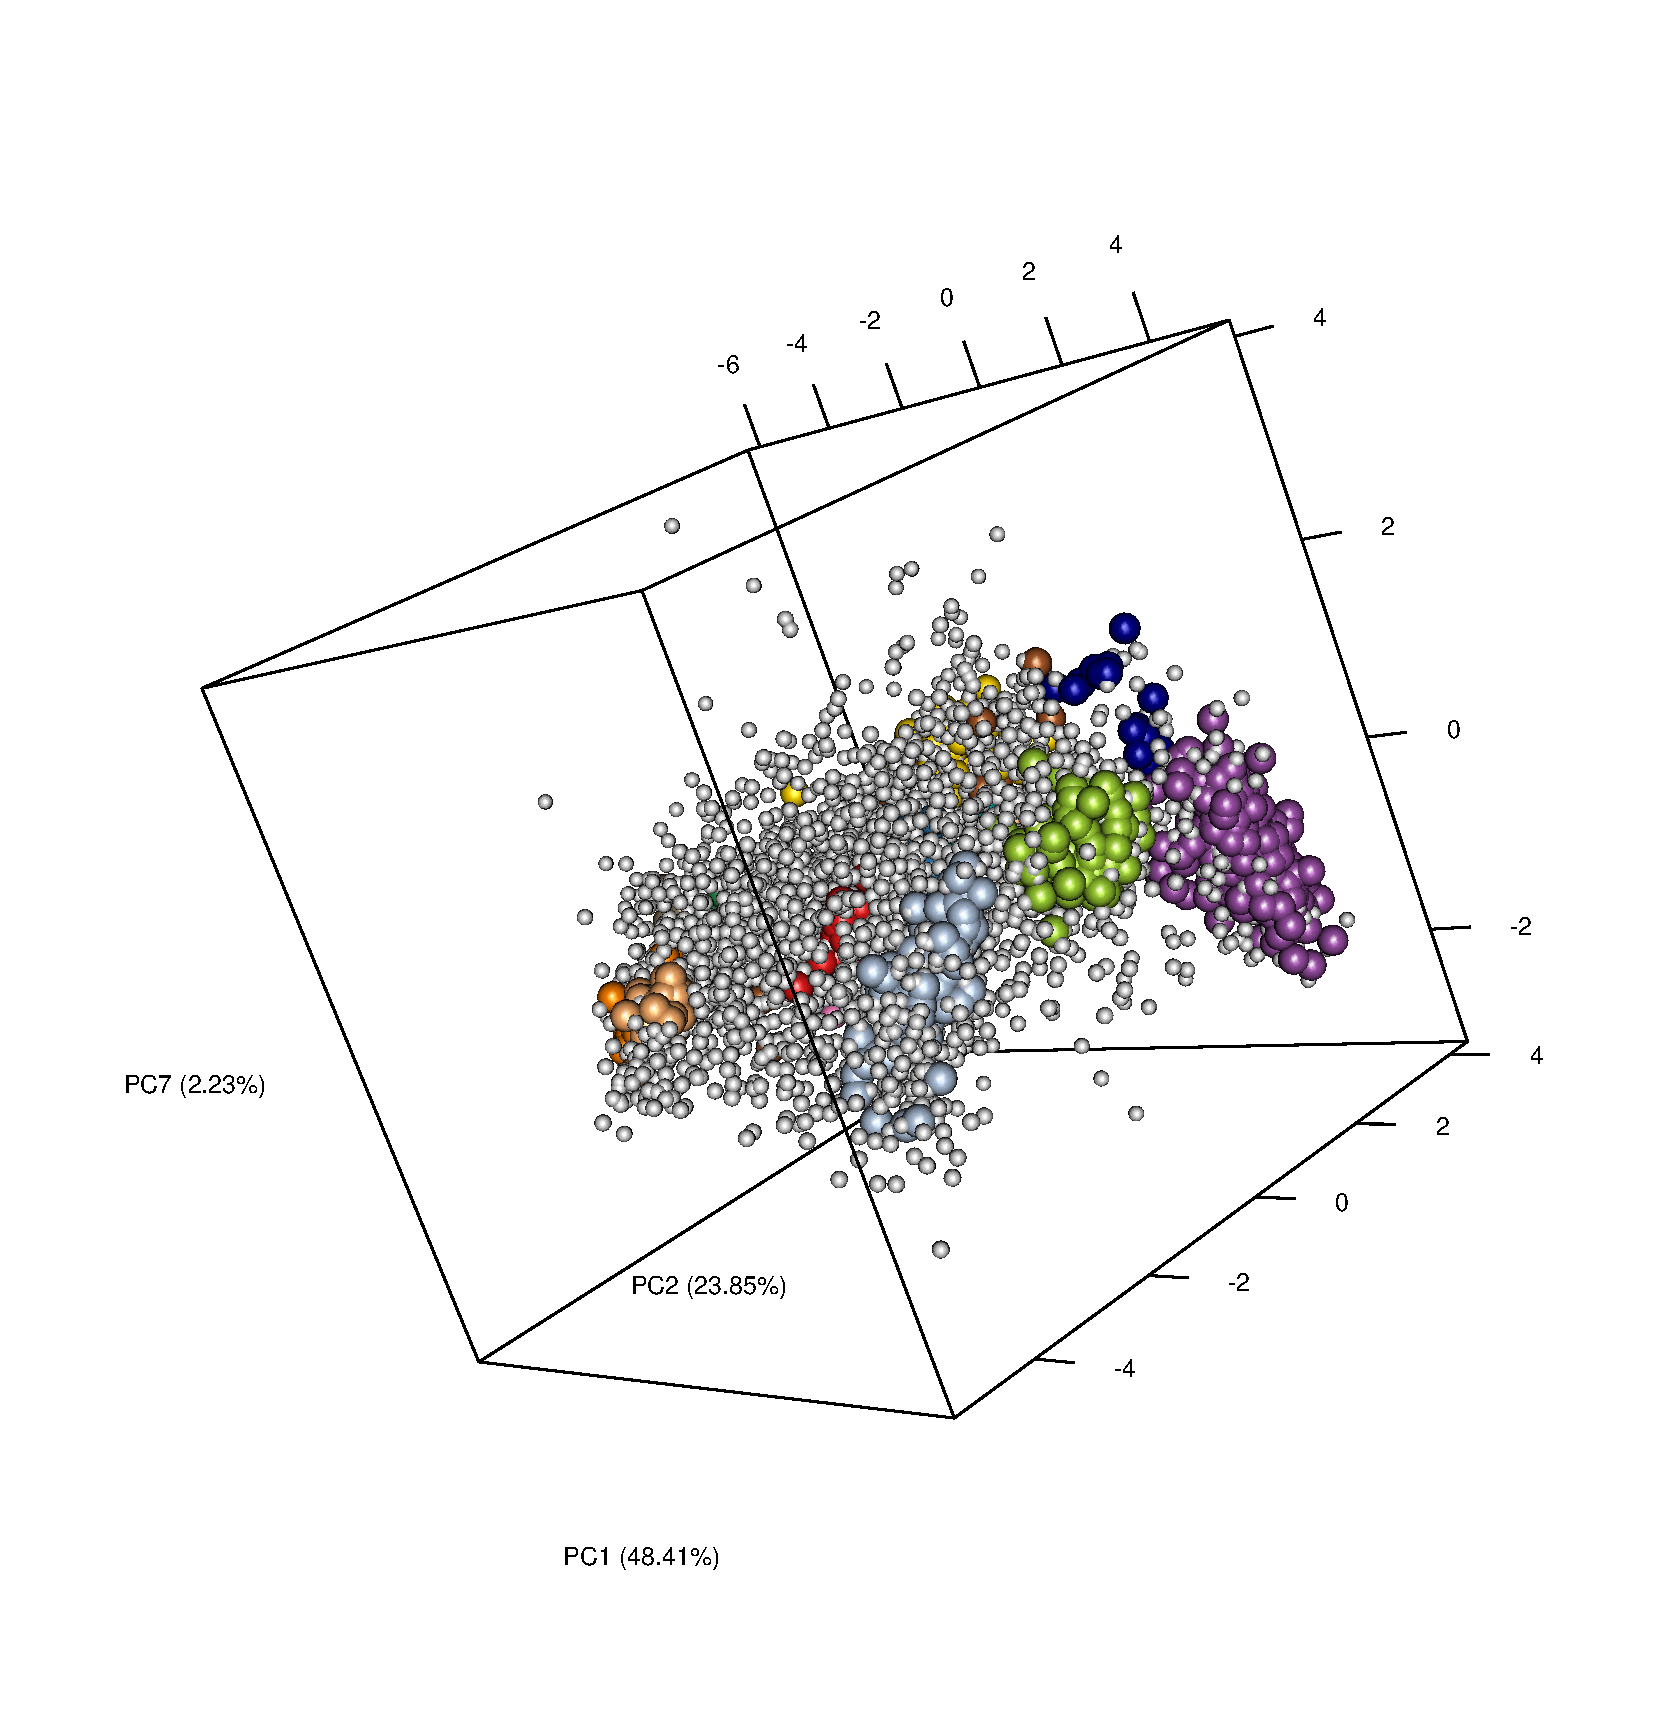
\includegraphics[width=.55\textwidth]{./Figures/plot3d.pdf}
  \caption{Using the \texttt{plot3D} function to visualise the
    \texttt{hl} dataset along PCs 1, 2 and 7. }
  \label{fig:plotmarkers3d}
\end{figure}

The default colours for plotting have been defined so as to enable the
differentiation of up to 30 classes. If more are provided, different
character symbols (circles, squares, ... and empty and solid symbols)
are used. The colours and the default plotting characters (solid dots
for the markers and empty circles for the features of unknown
localisation) can of course be changed, as described in the
\texttt{setStockcol} manual page.

As demonstrated in \cite{hyper} and illustrated in the PCA plot
(Figure \ref{fig:plotmarkers}), the Golgi apparatus proteins (dark
brown) display a dynamic pattern, noting sets of Golgi marker proteins
that are distributed amongst other subcellular structures, an
observation supported by microscopy.  As such, we are going to reset
the annotation of Golgi markers to unknown using the
\texttt{fDataToUnknown} function. It is often used to replace empty
strings (\texttt{""}) or missing values in the markers definition to a
common definition of \textit{unknown} localisation.

\begin{Schunk}
\begin{Sinput}
> hl <- fDataToUnknown(hl, from = "Golgi apparatus", to = "unknown")
> getMarkers(hl)
\end{Sinput}
\begin{Soutput}
organelleMarkers
           40S Ribosome            60S Ribosome      Actin cytoskeleton 
                     27                      43                      13 
                Cytosol   Endoplasmic reticulum                Endosome 
                     43                      95                      12 
   Extracellular matrix                Lysosome           Mitochondrion 
                     10                      33                     383 
    Nucleus - Chromatin Nucleus - Non-chromatin              Peroxisome 
                     64                      85                      17 
        Plasma membrane              Proteasome                 unknown 
                     51                      34                    4122 
\end{Soutput}
\end{Schunk}

Finally, in addition to \texttt{plot2D}, the \texttt{plot3D} function
allows to interactively explore a 3-dimensional plot of the data.

\subsection*{Features of interest}
In addition to adding annotation using the \texttt{addMarkers}
function, one can store specific sets of proteins by using the
\textit{Features of interest} infrastructure from the
\Biocpkg{MSnbase} package. If users have specific subsets of proteins
they wish to highlight in their data (possibly across multiple
experiments) they would first create a \texttt{FeaturesOfInterest}
object \hl{and then use the \textit{highlightOnPlot} function to 
visualise these}. For example, if we wanted to highlight \sout{a} 
proteins with the accession numbers Q8CG48, Q8CG47, Q8K2Z4, and Q8C156, 
which are some of the proteins known to form part of the 13S condensin complex, 
we \hl{would call the following code:}
\sout{would create a first create a \texttt{FeaturesOfInterest} object, and
subsequently highlight their location on a PCA plot with the
\texttt{highlightOnPlot} function.}



Users can also create several sets of \texttt{FeaturesOfInterest}
object and store them in a \texttt{FoICollection}.

It is also worthy of note that it is possible to search for a
specific protein of interest by \texttt{featureNames} or using any
identifying information found in the \texttt{fData} columns by using
the search box on the \texttt{pRolocVis} application part of the
\Biocpkg{pRolocGUI} package (see section on interactive
visualisation). This can be handy for quickly searching and
highlighting proteins on the fly, the disavanatge here is that
proteins can only be searched for a one-by-one basis.

\section*{Replication}

With the aim of maximising the sub-cellular resolution and,
consequently, the reliability in protein sub-cellular assignments, we
follow the advice in \cite{Trotter:2010} and combine replicated spatial
proteomics experiments as described above. Indeed, Trotter et
al. have shown a significant improvement in protein–organelle
association upon direct combination of single experiments, in
particular when these resolve different subcellular niches.

Direct comparisons of individual channels in replicated experiments
does not provide an adequate, goal-driven assessment of different
experiments. Indeed, due to the nature of the experiment and gradient
fraction collection, the quantitative channels do not correspond to
identical selected fractions along the gradient. For example, in the
table below (taken from \texttt{hl}'s \texttt{pData}) TMT channels
127C (among others) in both replicates originate from different sets
of gradient fractions (gradient fractions 7 - 9 and 8 - 9 for each
replicate, respectively). Different sets of gradient fractions are
often pooled to obtain enough material and optimise acurate
quantitation.

